\chapter{Konfigurationsraum}

% https://cs.stanford.edu/people/eroberts/courses/soco/projects/1998-99/robotics/definitions.html

Bei einer Roboterlänge und -breite größer als eins können Punkte im Occupancy Grid nicht erreicht werden, ohne mit den Roboterdimensionen Hindernisse oder Grenzen zu überdecken. 
Aus diesem Grund wird die Bewegung des Roboters im Occupancy Grid in eine Punktbewegung im sogenannten \textit{Konfigurationsraum} transformiert.
In diesem Raum entsprechen die Roboterdimensionen einem Punkt (Roboterlänge = Roboterbreite = $1$), was die Überdeckung von Hindernissen und Grenzen verhindert.

Zur Berechnung des Konfigurationsraums wird jedes Hindernis im Occupancy Grid um die Roboterdimensionen erweitert.
Aufgrund der variablen Roboterdimension ändern sich die überdeckten Koordinaten im Occupancy Grid je nach aktueller Rotation.
Ansätze in der Literatur schlagen deshalb vor, unabhängig von der aktuellen Rotation des Roboters, jedes Hindernis in X- und Y-Richtung um einen Kreis mit maximaler Roboterdimension als Radius zu vergrößern.

XYZ (TODO) schlägt einen restriktiveren Ansatz vor, um möglichst wenig Koordinaten um das Hindernis im Konfigurationsraum zu erweitern.
Dazu wird die Roboterrotation in diskrete Schritte unterteilt. Die Variable \texttt{rotation\_step} gibt als Teiler von 360° an, um wie viel Grad sich der Roboter pro Bewegungsschritt drehen kann.
Somit sind $\texttt{rotations} = (360 \text{\textdegree} \div \texttt{rotation\_step})$ unterschiedliche Ausrichtungen des Roboters um den Ankerpunkt möglich.

\begin{figure}[h!]
	\centering
	\footnotesize
	\centerline{\resizebox{0.7\linewidth}{!}{\input{bilder/rotation-steps_latex.pdf_tex}}}
	\caption{Bei $\texttt{rotation\_step}=45$° ergeben sich $(360 \text{\textdegree} \div 45) = 8$ Rotationszustände.}
\end{figure}

Für das Robotermodell wird eine Maske als 2D-Array (\texttt{robot\_length}$*$\texttt{robot\_width}) erstellt und für jeden Rotationsschritt mit \texttt{sklearn.rotate()}\footnote{Mögliche Artefakte und Interpolation der Matrixrotation müssen manuell korrigiert werden.} gedreht.
Für jede der $(360 \text{\textdegree} \div \texttt{rotation\_step})$ möglichen Rotationen wird ein \textit{erweitertes Occupancy Grids} generiert. Dazu werden Hindernisse sowie Grenzen des ursprünglichen Occupancy Grids um die rotierte Maske erweitert.
Beispielsweise Rotation um 45° ...

\begin{figure}[h!]
	\centering
	\footnotesize
	\centerline{\resizebox{0.9\linewidth}{!}{\input{bilder/robot-mask_latex.pdf_tex}}}
	\caption{Erzeugung eines erweiterten Occupancy Grid für eine Rotation um $45$°}
\end{figure}


Die erweiterten Occupancy Grids werden zum Konfigurationsraum \texttt{configuration-space[rotation][y][x]} mit den Dimensionen $\texttt{rotations} * \texttt{occupancy\_grid\_length} * \texttt{occupancy\_grid\_width}$ zusammengefasst. Für die Dimension \texttt{[rotation]} gilt:
\begin{itemize}
\item $\text{[}(\texttt{rotation} + 1) \mod \texttt{rotations]}$ $\widehat{=}$ Rotation um \texttt{rotation\_step} im Uhrzeigersinn
\item $\text{[}(\texttt{rotation} - 1) \mod \texttt{rotations]}$ $\widehat{=}$ Rotation um \texttt{rotation\_step} gegen den Uhrzeigersinn
\end{itemize}

\begin{figure}[h!]
	\centering
	\footnotesize
	\centerline{\resizebox{1\linewidth}{!}{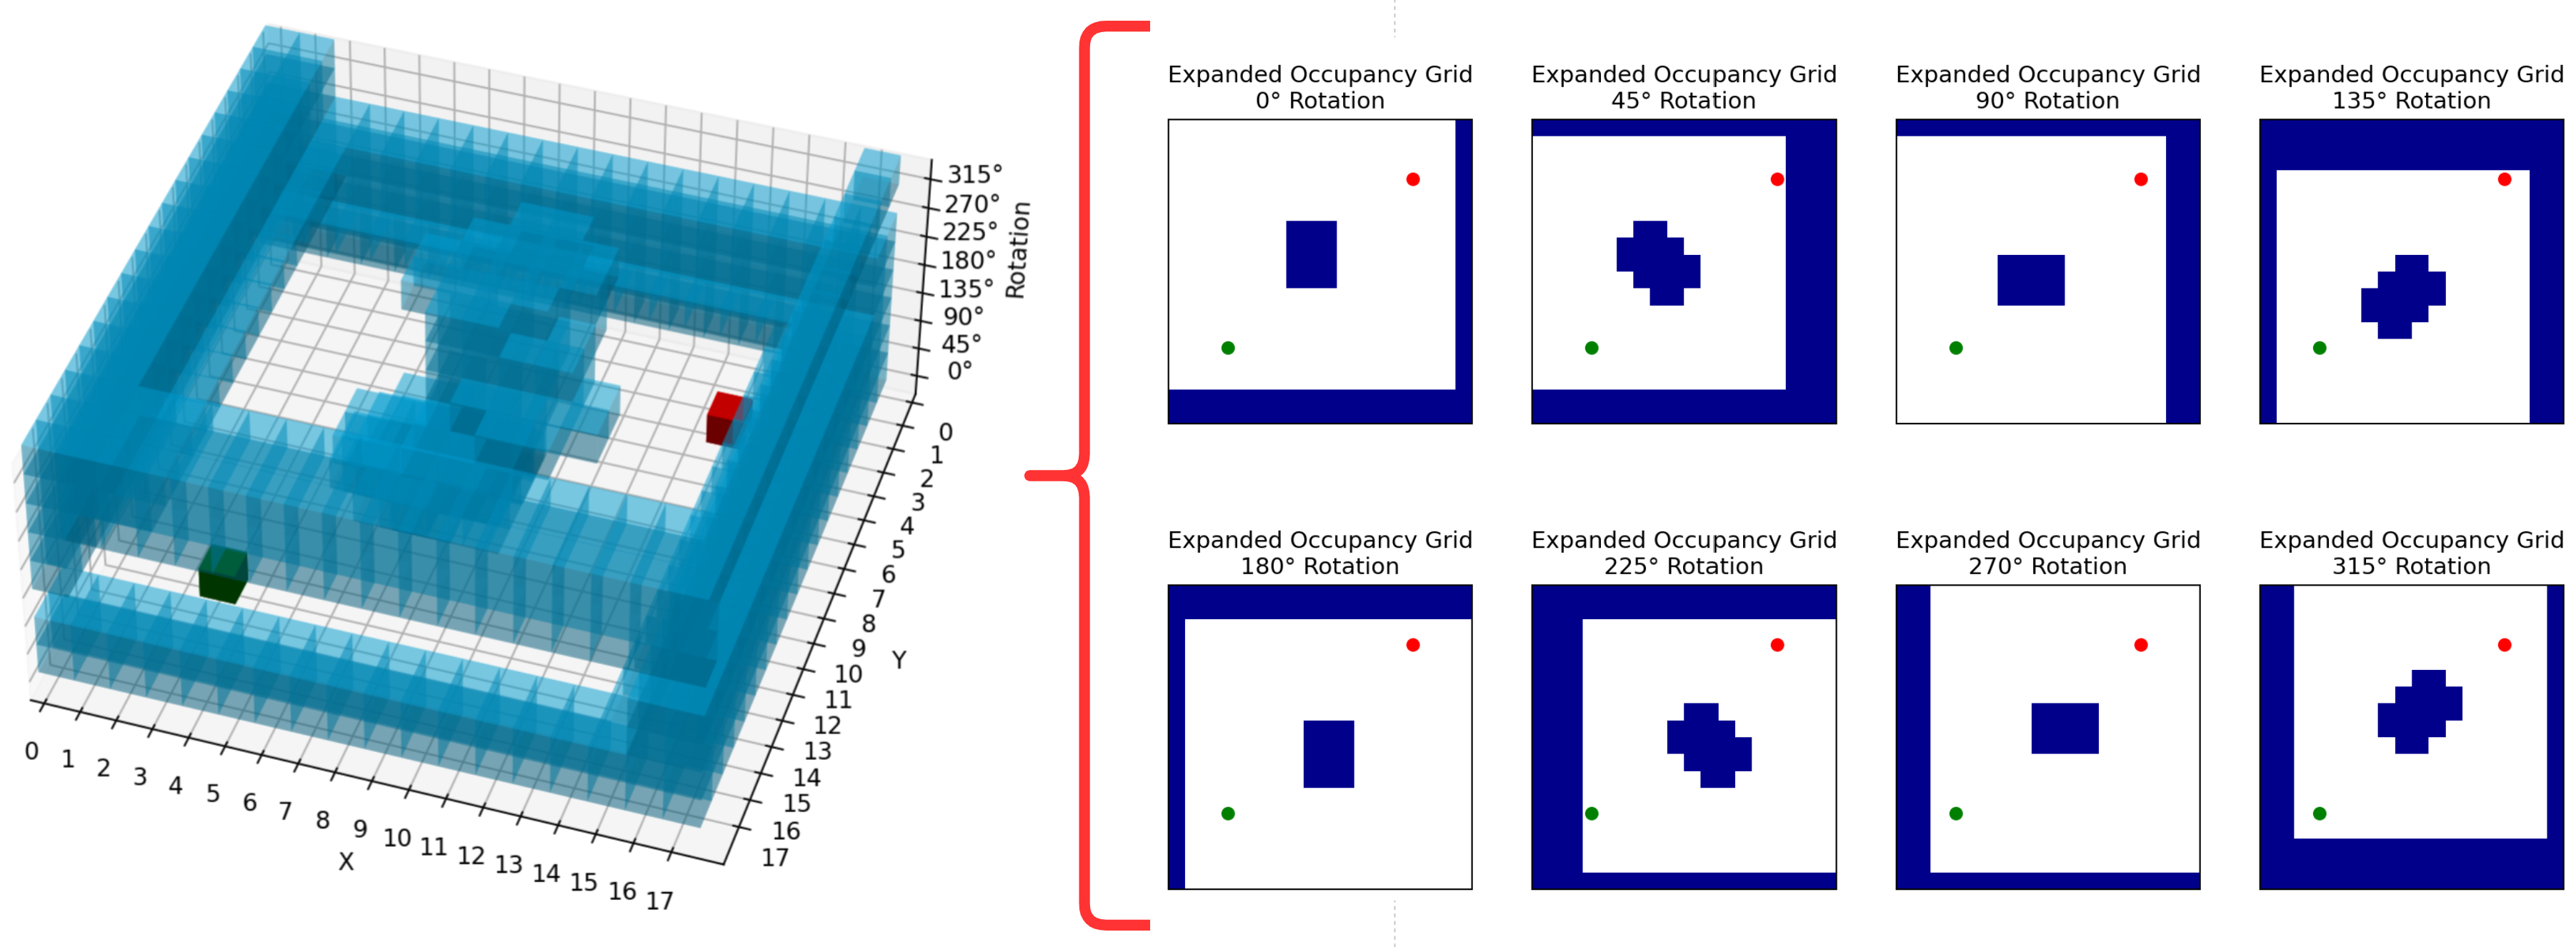
\includegraphics{bilder/configuration-space.png}}}
	\caption{Die erweiterten Occupancy Grids bilden den Konfigurationsraum}
\end{figure}

Dieser 3D Konfigurationsraum ermöglicht die kollisionsfreie Translation und Rotation bei minimalem Verbrauch freier Koordinaten.
